\documentclass{kththesis}



\titleformat
{\chapter}
[display]
{\normalfont\Large\bfseries}
{Kapitel \thechapter}
{0.5ex}
{}
[]



\usepackage{blindtext} % This is just to get some nonsense text in this template, can be safely removed

\usepackage[parfill]{parskip}
\usepackage{caption}
\usepackage{multirow}
\usepackage{pdfpages}
\usepackage{graphicx}
\usepackage[toc,page]{appendix}
\graphicspath{ {./images/} }
\usepackage{mathtools}
\usepackage{csquotes} % Recommended by biblatex
\usepackage{biblatex}
\addbibresource{references.bib} % The file containing our references, in BibTeX format


\title{This is the English title}
\alttitle{Detta är den svenska översättningen av titeln}
\author{Osquar Studnt}
\email{osquar@kth.se}
\supervisor{Lotta Larsson}
\examiner{Lennart Bladgren}
\programme{Master in Computer Science}
\school{School of Electrical Engineering and Computer Science}
\date{\today}

\begin{document}


% Frontmatter includes the titlepage, abstracts and table-of-contents
\frontmatter

\titlepage
\begin{otherlanguage}{swedish}
  \begin{abstract}
I dagsläget finns det en mängd utmaningar och svårigheter inom den traditionella UX-designprocessen. Dessa utmaningar har en påverkan på hur tidskrävande och kostsam en UX-designprocess kan vara. Några av dem är att få prototyper att likna slutprodukten med avseende på funktionalitet, användargränssnitt och användarupplevelsen och att UX-designers sällan får tillräckligt med input från utvecklare vad det gäller funktionella begränsningar. Det finns även svårigheter vid visualisering av data, mer specifikt strömmande data. Svårigheten ligger i att göra informationen i data så lättförståelig för användaren som möjligt och att möjliggöra användaren att få ut önskad information. Svårigheten beror på en mängd faktorer som datats komplexitet samt hastigheten och mängden data som strömmar in. 

För att undersöka dessa svårigheter togs det fram en UX-designprocess vid användning av datavisualiseringsverktyget Kibana, som är en del av Elastic Stack. Elastic stack är ett verktyg som består av fyra projekt som hämtar, hanterar, tillfälligt lagrar och visualiserar data. För att kunna utvärdera och bedöma UX-designprocessen vid användning av Kibana skapades en interaktiv dashboard som presenterade Transportstyrelsens data från betalstationer. Under detta projekt togs en UX-designprocess fram där prototypskapandet och testningen optimerades då följande krav var uppfyllda: det som skulle visualiseras var data som var kompatibel med Kibana, systemet skulle vara fulländat innan skapandet av UI-element skulle påbörjas och det krävdes inte mycket modifiering av UI-element. Om kraven inte uppfylldes visade det sig att Kibana har en del begränsningar vad det gäller vad som kan visualiseras och hur visualiseringen kan modifieras. 

\textbf{Nyckelord}

\textit{Kibana, Elastic Stack, UX-designprocess, UX, Användarupplevelse}

 \end{abstract}
\end{otherlanguage}
 

\begin{abstract}

In the current situation there are a lot of challenges and difficulties in the traditional UX-design process. These challenges have an impact on how time consuming and costly a UX-design process can be. Some of them are to get prototypes to match the end product with regard to functionality, user interface and user experience and UX-designers rarely get enough input from developers regarding functional limitations. There are also difficulties in visualizing data, more specifically streaming data. The difficulty lies in making the information in the data as easy to understand as possible for the user and to enable the user to obtain the desired information. The difficulty is due to a variety of factors such as data complexity as well as the speed and amount of data flowing in.

To investigate these difficulties, a UX-design process was developed using the data visualization tool Kibana, which is part of Elastic Stack. Elastic stack is a tool consisting of four projects that retrieve, manage, temporarily store and visualize data. In order to evaluate and assess the UX design process when using Kibana, an interactive dashboard was created that presented data from Swedish payment stations. During this project, a UX-design process was developed where prototype creation and testing were optimized when the following requirements were met: the data that would be visualized was compatible with Kibana, the system would be completed before the creation of UI-elements would begin and no bigger modification of UI-elements was required. If the requirements were not met, it appeared that Kibana has some limitations as to what can be visualized and how much visualizations can be modified.

\textbf{Keywords}

\textit{Kibana, Elastic Stack, UX-design process, UX, User Experience}

\end{abstract}

\chapter*{Förord}
Detta projekt är ett resultat av ett examensarbete inom datateknik på Kungliga Tekniska Högskolan, på uppdrag av företaget ÅF Digital Solutions AB. Arbetet har utförts av Christina Ntis och Neira Causevic på heltid under perioden mars 2018 - juni 2018.

Text som är i kursiv stil i denna rapport är termer på engelska som inte var lämpliga för översättning till svenska.

Vi skulle vilja tacka alla inblandade parter i detta examensarbete på ÅF och KTH. Stort tack till, Martin Neumann, vår handledare på ÅF för all kunskapsdelning, stöd och rådgivning. Tack även till Anders Lindström som var vår handledare på KTH för all hjälp med detta examensarbete. 

\tableofcontents


% Mainmatter is where the actual contents of the thesis goes
\mainmatter


\chapter{Inledning}

För 30 år sedan uppstod konceptet användarupplevelse, mer känt som UX, som står för engelskans User Experience. Det är kvalitén på upplevelsen och erfarenheten som användaren får vid interaktion med en viss produkt, ett system eller en tjänst. För att ge användare en bra användarupplevelse bör användargränssnittet, d.v.s. det grafiska gränssnittet, vara användarvänligt. Detta innebär att gränssnittet ska vara lätt att använda och förstå samt uppfylla de avsedda användarnas behov och hjälpa användaren att utföra den önskade uppgiften. 

Dock är det inte alltid lätt att skapa användargränssnitt för produkter, speciellt när det gäller att visualisera strömmande data. Svårigheten ligger i att göra informationen i data så lättförståelig för användaren som möjligt och att möjliggöra användaren att få ut önskad information. Svårigheten beror på en mängd faktorer som datats komplexitet samt hastigheten och mängden data som strömmar in.

För att ta fram användargränssnitt bör en UX-designprocess följas, dock finns det i dagsläget många utmaningar i denna designprocess. Några av dessa svårigheter är att prototyper sällan är lika slutprodukten vad det gäller funktionalitet, användargränssnitt och användarupplevelsen. Dessutom får UX-designers sällan tillräckligt med input från utvecklare vad det gäller funktionella begränsningar. Det utgör ett problem då användaren skulle kunna testa funktionalitet som inte är möjlig att skapa i systemet eller att användaren missar att testa funktionalitet som är möjlig att skapa. Anledning till varför användargränssnittet skulle kunna variera i prototypen och slutprodukten är att UX-designers ofta inte använder samma visualiseringsverktyg som produktutvecklarna. Kombinationen av att utseendet och funktionaliteten kan variera skulle i sin tur leda till att användarupplevelsen vid testning av prototypen skulle variera från användarupplevelsen vid användning av slutprodukten. 

Ytterligare en svårighet som finns vid framtagandet av interaktiva prototyper är att detta kan vara väldigt tidskrävande för en UX-designer. Detta eftersom resultatet av varje användarinteraktion som ska finnas i slutprodukten även skulle behöva tas fram för prototypen. Därför leder detta problem, samt de ovan nämnda, till att extra tid måste läggas ned av UX-designern vilket även ökar kostnader. 

I detta projekt användes därför ett verktyg där produktframtagningen och prototypskapandet kunde ske samtidigt. Syftet var att utvärdera designprocessen vid användningen av det verktyget jämfört med den vanligen använda designprocessen. Verktyget skulle användas för hämtning, tillfällig lagring och visualisering av data. Det fanns en mängd olika verktyg för detta som t.ex. Elastic Stack, Loggly och Scalyr. Eftersom Elastic Stack säger sig vara “en världsledande mjukvaruleverantör för att göra strukturerad och ostrukturerad data användbar i realtid för användarfall som sökning, loggning, säkerhet och analys” [1] valdes detta verktyg. I samma artikel presenteras statistiken att Elastic Stack har över 100 miljoner nedladdningar vilket visar på att det är extremt populärt och använt. Dessutom var Elasticsearch, som är sökmotorn i Elastic Stack och möjliggör lagring, sökning och analys av stora mängder data i nära real-tid, den mest populära sökmotorn enligt en rakning av sökmotorer som gjorts på DB-Engines i Maj 2018 [2]. Eftersom Kibana används för visualisering av data som finns i Elasticsearch är det även möjligt för alla Elasticsearch användare att använda Kibana vilket skulle innebära en stor mängd potentiella användare av Kibana. Under projektets gång låg fokus på Kibana eftersom det är visualiseringsverktyget i Elastic Stack.

Dataströmmen som användes som exempeldata vid visualiseringen var från Transportstyrelsens öppna databas gällande betalstationer i Sverige. Detta möjliggjorde en visualisering av trafik där användare kunde få information som t.ex. antal fordon som passerade ett valt område, fördelning av fordonstyper, var fordonsägare som åkte igenom valda betalstationer bodde m.m.

\section{Målsättning}
Detta arbete syftar till att undersöka om, och hur Kibana kan förbättra UX-designprocessen. Ett av målen i det här projekt var därför att ta fram viktiga problem och eventuella brister inom UX-designprocessen och undersöka dessa. Det skulle även skapas en produkt med hjälp av Elastic Stack där Kibana skulle användas som visualiseringsverktyg. Framtagningen av produkten gjordes för att kunna uppfylla det huvudsakliga målet med projektet vilket var en UX-designprocess som togs fram vid användning av Kibana. Den skulle sedan utvärderas av erfarna UX-designers för att jämföras med den traditionella UX-designprocessen. 

Projektet skulle ytterligare delas upp i följande mer detaljerade delmål:

\begin{itemize}

\item Identifiera problem och brister inom UX-designprocessen. 

\item Bedöma UX-designprocessen vid användning av Kibana baserat på utvärderingar av erfarna UX-designers. 

\item Bedöma kommunikationen mellan Agila utvecklare och UX-designers baserat på projektdeltagarnas erfarenhet av båda rollerna under UX-designprocessen vid användning av Kibana.

\item För att kunna utvärdera och bedöma UX-designprocessen vid användning av Kibana ska en interaktiv dashboard skapas med hjälp av Kibana som presenterade Transportstyrelsen data från betalstationer.

\begin{itemize}
\item Utforska slutanvändare och ta fram deras behov och krav.
\item Ta fram lösningar som uppfyller dessa behov och krav.
\item Implementera lösningarna i en interaktiv dashboard i Kibana 
\item Testa produkten mot slutanvändare genom djupintervjuer. 
\item Upprepa ovanstående steg tills produkten blivit accepterad av slutanvändaren.
\end{itemize}

\item Förbereda data för visualisering.
\begin{itemize}
\item Skapa en webbtjänst som skulle hämta data från Transportstyrelsen.
\item Modifiera data så att de skulle bli kompatibla med Kibana.
\end{itemize}

\end{itemize} 

\section{Avgränsningar}
Data som skulle användas för analys och visualisering skulle vara data från Transportstyrelsens betalstationer. Skapandet av webbapplikationen, analys och visualisering av data skulle göras med hjälp av Elastic Stacks \textit{open-source}projekt: Logstash, Elasticsearch och Kibana.  

\chapter{Teori och bakgrund}

Detta kapitel presenterar en bakgrund och teorier till hur ett användargränssnitt designas med användarupplevelsen, användargränssnittet, utmaningar i processen och strömmande data i fokus. Det tar även upp Elastic Stack som är verktyget som användes i projektet.

\section{Användarupplevelse och användargränssnitt} 
I detta avsnitt kommer termerna användargränssnitt och användarupplevelse presenteras. Även termernas betydelse till mjukvaruprodukter och tillämpning tas upp.

\subsection{Bakgrund} 

Den första datorn med ett grafiskt användargränssnitt var Xerox PARC och skapades 1973 [3]. Det hade bilder, listrutor och kryssrutor. Innan detta var användaren tvungen att interagera med en dator enbart via ett kommandoradsgränssnitt. Efter det första grafiska användargränssnittet har konceptet undersökts och utvecklats mycket och blivit en nödvändig del av en produkt. Användargränssnittet är inte bara ett grafiskt användargränssnitt, det är användbarheten av en produkt för användaren.

I och med utvecklingen av teknik, och den ständiga ökningen av andelen människor som använder teknikprodukter, uppstod aspekter av produkter som inte tidigare undersökts såsom användarupplevelse. Konceptet User Experience (UX) introducerades först 1990-talet av Donald Norman [4]. Innan termen User Experience introducerades hänvisade människor till detta koncept som "critical aspects of human interface research and application".

\subsection{Användarupplevelse}
 
Enligt definitionen framtagen av främst Donald Norman i artikeln “The definition of User Experience (UX)” [5] är användarupplevelse kvaliteten på upplevelsen och erfarenheten som användaren får vid interaktion med en viss produkt, ett system eller en tjänst. Det handlar om utvecklingen av kvaliteten på användarens interaktion med dessa tjänster. Det är ett koncept som utforskar varje stadie som användaren måste gå igenom vid användning av en tjänst, system eller produkt. En del av dessa aspekter är processen att hitta produkten, handlingar för att interagera med produktens gränssnitt, känslomässiga förändringar som kan uppstå under produktanvändning och vilket intryck produkten lämnar efter att den har använts. Det innefattar även allt som berör användarens erfarenhet av produkten även när användaren informerar en annan person om produkten. En produkt måste uppfylla användarens behov utan att skapa en dålig upplevelse för denne. Dessutom måste produkterna avge enkelhet och elegans för att kunna erbjuda användaren tillfredsställelse. 

Användarupplevelse är en mycket komplicerad process som överstiger vad användaren trodde sig vilja och utforskar djupt det bästa sättet att förbättra användbarheten hos produkten och öka tillfredsställelsen. Under processen undersöks de positiva känslorna användaren har vid interaktion med produkterna och sätt att förbättra dem enligt rapporten “UX Gymnastics: Representation of UX Theory and Concepts through Full Body Movement” [6]. Detta koncept bildas således på mätningar av användarens attityder, preferenser och beteende. 

I boken “Measuring the User Experience” [7] av Tom Tullis och Bill Albert förklaras det att användarupplevelsens stora inflytande på användaren har fått många företag att tillägna avdelningar som är dedikerade till att undersöka och förbättra användarupplevelsen av sina produkter. Anledningen till att användarupplevelse är så viktigt för producenterna är att när en produkt saknar användarupplevelse eller inte har tillräckligt med användarupplevelse, påverkar det radikalt försäljningen av produkten. 

\subsection{Användargränssnitt}
Användargränssnittet, även kallat UI efter engelskans User Interface, är den del av en systemprogramvara som användaren kan se, höra, röra eller prata med enligt boken “The Essential Guide to User Interface Design: An introduction to HUI Design” [8]. Det är indelat i två aspekter, ett är användarinmatningen och ett är systemutmatningen. Inmatningen är det sätt som användaren interagerar med systemet och kan vara via tangentbordet, musen, pekskärmen eller rösten. Utmatningen är hur användaren kommer att få ett svar från systemet och det främsta exemplet på det i dagens samhälle är en bildskärm. Användargränssnittsdesign kommer från en studie kallad människa-datorinteraktion som är studien, planeringen och designen av hur människor och datorer kommunicerar för att uppfylla användarens behov.

Ett bra användargränssnitt är ett gränssnitt som är lätt att använda och förstå. Det uppfyller den avsedda användarens behov och hjälper användaren att utföra den önskade uppgiften. Det visas att om användaren inte är nöjd med en ansökan efter första användningen finns det 80 \% möjlighet att användaren slutar använda applikationen [9]. Därför är det viktigt att säkerställa att användargränssnittet är bäst under utvecklingen med hjälp av designprocessen i användargränssnittet.

Vid design av ett användargränssnitt bör principer inom Människa-Dator Interaktion, förkortat MDI, följas. Det är studien, planeringen och designen av hur människor och datorer interagerar med varandra så att personens behov är uppfyllda på det mest effektiva sättet [8]. För att kunna göra detta gäller det att förstå de två komponenterna inom MDI - människan och datorn. För att förstå människan bör man se på psykologiska och sociala aspekter samt mänskliga fel och man bör veta och känna till den tänkta användaren för produkten. För att förstå datorn är begränsningar, kapacitet, verktyg och plattformar i fokus.

\subsection{Ergonomiskt och biologiskt perspektiv}

I boken “Arbete och teknik på människans villkor” [10] lyfts det fram att för att skapa produkter som underlättar människors användning av datorer och förenkla förståelsen av presenterade data måste det tas hänsyn till de fysikaliska faktorerna som kan påverka människans interaktion med teknologiska produkter. Eftersom en väldigt stor del av informationen som finns i vår omgivning tas in av människor genom synen så är den en stor faktor vid människans interaktion med en teknologisk produkt som till exempel en webbapplikation. Detta betyder att vid skapandet av teknologiska produkter måste synergonomiska aspekter betraktas. 

Synergonomiska aspekter handlar om att presentera data på ett sådant sätt så att de inte belastar användarens ögon. Några exempel på detta kan vara att skapa bra kontraster på bakgrunden och texten i en webbapplikation, ha tydliga menyer som användaren kan få information från och ha data presenterade på ett organiserat sätt så att användaren får korrekt information utan att tröttas ut. Denna aspekt är väldigt viktig eftersom den förhindrar användarens ögontrötthet och ger en mer effektiv informationsöverföring. 

Det är inte tillräckligt att endast presentera information, presentationen måste även underlätta hjärnans tolkningsprocess vid inmatning av data för att kunna dra slutsatser och dra nytta av informationen som presenteras. Människans erfarenheter av användning av produkter bidrar mycket till tolkningsprocessen och därför är det viktigt att följa vissa standarder för visualiseringsmetoder vid presentation av data. Ett exempel på detta kan vara användning av kugghjulsikoner för att hänvisa till inställningar, en papperskorg för att ta bort någonting och en penna för att ändra någonting. 

Något som också är viktigt att tänka på då användarens förståelse av dataströmmen är i fokus är att kunna möjliggöra en fullständig presentation av det allmänna läget men också ha stöd för att kunna se detaljer i datat enligt rapporten “A visual analytics agend” [11]. Man bör även göra det möjligt för användaren att integrera olika typer av information och data till en enda presentation för att öka förståelsen av det som presenteras.

En ganska stor del av befolkningen är färgblinda, vilket betyder att de kan ha svårt att urskilja alla eller vissa färger [12]. Det är en utmaning att kunna skapa teknologiska produkter som ska kunna användas även av människor med detta handikapp [10]. Detta kan göras genom att undvika vissa färgkombinationer, där rött och grönt är de vanligaste kombinationerna som människor är färgblinda för.


\subsection{UX-designprocess}


Inom begreppet MDI tillhör interaktionsdesign som har som mål att öka människors förståelse över vad som kan göras, vad som sker och vad som precis hänt. För att kunna göra detta och försäkra en positiv användarupplevelse av produkten som designas så ska principer inom psykologi, design, konst och känsla följas. Kraven inom detta område är att försäkra att människors behov är mötta, att den resulterande produkten är förståelig, lätt och naturlig att använda och det ska vara svårt att göra fel. Dessutom ska användaren kunna utföra önskade uppgifter och upplevelsen ska vara positiv och njutningsbar för användaren.           

\captionsetup[figure]{name=Figur}

\begin{figure}[h]
\centering
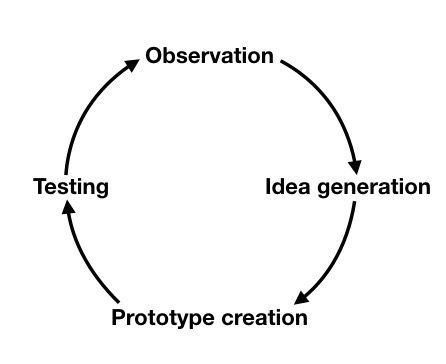
\includegraphics[width=0.5\textwidth]{PrototypeCreation}
\caption{Redogörelse för de fyra stegen för optimal design.}
\end{figure}

Enligt upphovsmannen till UX, Donald Norman [13] består människa-centrerad designprocess av fyra steg som itereras enligt figur 2.1. I boken “The design of everyday things” [14] tas det upp att denna metod brukar även kallas för “the spiral method” och syftar på att leverera framsteg vid varje iteration. Dessa fyra steg är: 

\begin{enumerate}
\item Observation: handlar om att undersöka och förstå problemet. Det handlar om att undersöka och observera slutanvändaren för att kunna förstå deras behov, intresse och motivationer. Det görs genom att observera, lyssna och intervjua användarna. I detta steg bestäms designkraven. Med hjälp av undersökningen kan designern skapa personas, vilket är användarprofiler som representerar slutanvändarna och inkluderar information om deras motivationer, mål, behov och förväntningar [15]. Dessa användarprofiler skapas i början av ett projekt och kan ändras i ett senare skede vid behov. [16]

\item Idéskapande: går ut på att baserad på designkraven hitta lösningar som uppfyller dessa krav. Tillvägagångssättet för den delen av designprocessen görs enligt följande tre steg:
\begin{itemize}
\item att vara kreativ och frambringa många idéer,
\item att undvika kritisera dessa idéer, att vara kreativ utan hänsyn till begränsningar,
\item att ifrågasätta allting, även det uppenbara. 
\end{itemize}

\item Prototypskapande: går ut på att skapa första utkastet till produktens användargränssnitt. Att experimentera med olika designs, demonstrera användargränssnittet till ledningen och kontrollera om produkten är funktionell och användbar är del av detta steg. En känd prototypteknik är “Wizard of Oz”. I denna teknik skapar prototyper som efterliknar stora och komplexa system innan de är gjorda. Det ger möjligheten att presentera hur produkten skulle interagera med användaren. 

\item Testning: handlar om att observera interaktionen mellan prototypen och användaren. Det kan även göras genom demonstration av olika versioner av användargränssnittet till användarna, intervjua användaren, ställa frågor, använda sig av enkäter för att kunna identifiera svårigheter med användargränssnittet.
 
\end{enumerate}

Genom iterationen av dessa fyra steg möjliggörs ständigt förbättring av användargränssnittet. När kraven för användargränssnittet är specificerade det skapas en prototyp och den testas för att säkerställa att dessa krav uppfylls. UX designern får återkoppling från personerna som testar användargränssnittet och baserad på det kan en ny iteration börja. Efter varje iteration förbättras användargränssnittet, den blir mer riktat till slutanvändare och kvalitet av produkten ökas. [14]

\subsection{Utmaningar i UX-designprocessen}

I rapporten “User experience prototyping - a literature review” [17] diskuterar Tuomas Nissinen fidelity-aspekten av prototyper som tas fram under designprocessen. Fidelity definieras som det koncept som betecknar hur lik en prototyp är med slutprodukten. Det finns prototyper som tillämpar olika nivåer av fidelity där nivåerna kategoriseras enligt: low-fidelity prototyper, high-fidelity prototyper, mixed-fidelity prototyper och multi-fidelity prototyper. Dessa prototyper används vid olika situationer då kostnad, tid och syfte kan variera. Low-fidelity kan göras både med papper och penna och på datorn. Den syftar på att presentera ett koncept eller idé istället för att presentera funktionaliteten av hela systemet. Dessa prototyper brukar göras tidigt i designprocessen, är snabba och har extremt låg kostnad. Några nackdelar med dem är att de har begränsningar angående användbarhet och testning. En high-fidelity prototyp har däremot all funktionalitet av systemet samt stödjer användarinteraktion med det. Den är väldigt lik slutprodukten och är väl anpassad för testning. Stödet för interaktiv funktionalitet gör dessa prototyper speciellt användbara vid upptäckt av användbarhetsproblem. Nackdelarna är dock att de är mycket mer tidskrävande än low-fidelity prototyper samt att de är mer kostsamma att ta fram. High-fidelity prototyper är inte heller anpassade för visualisering av komplex funktionalitet. Mixed-fidelity och multi-fidelity prototyper är blandningar av de tidigare nämnda prototyperna. Enligt Tuomas Nissinen är skapandet av interaktiva prototyper en stor utmaning för designers. Detta eftersom det skulle vara väldigt tidskrävande att stödja interaktiv funktionalitet i low-fidelity prototyper eller implementera komplex funktionalitet i high-fidelity prototyper.

Enligt Kate Pernice i Nielsen Norman Group [18] måste en prototyp av ett användargränssnitt testas för att möjliggöra bedömningen av dess användbarhet. Vid testning av prototypen måste alltså användaren få gensvar från prototypen vid handlingar och detta kan göras på två sätt. Det ena sättet går ut på att en person som är bekant med designen ska ge gensvar till användare testar prototypen och en sådan prototyp kallas för statisk.  Det andra sättet är genom att implementera dessa gensvar vilket resulterar i en interaktiv prototyp. Skapandet av en sådan prototyp kan bli tidskrävande. Även Pernice lyfter fram de områden där fidelity kan variera vilka är interaktivitet, innehåll, kommando och visuellt. 

Vid utveckling av design till ett system, en tjänst eller en produkt krävs även ett team som ska utveckla det som ligger bakom designen och utgör funktionaliteten. Teamet är delar av större organisationer och enligt en undersökning gjord av Project Management Institute [19] använder sig 71 \%, av organisationer som deltog i undersökningen, av Agila metoder ibland, ofta eller alltid. När UX-designers ska följa Agila metoder kan det bli problematiskt. I en rapport skriven av Michael Budwig, Soojin Jeong och Kuldeep Kelkar vid namn “When User Experience Met Agile: A Case Study” [20] beskrivs svårigheter som kan uppstå vid denna situation. På grund av att UX-teamet behöver utveckla design innan utvecklingsteamet har utvecklat det bakomliggande systemet kunde inte UX-teamet ofta få nödvändiga inputs från utvecklingsgruppens medlemmar. Vid uppkomsten av problem och nya krav för produkten i sprinter är UX-teamet tvungna att hantera både nya dem problem och kvar som har uppkommit och samtidigt leverera sina primära projekt i tid. Detta kan orsaka en stressig och negativ arbetsmiljö för UX-teamet. 

I rapporten “Experience Prototyping” [21] påpekas att designers borde fokusera på att utforska genom att göra, eftersom även små ändringar i ett användargränssnitt kan ha stora konsekvenser i den slutliga användarupplevelsen. Rapporten lyfter även fram betydelsen av skapandet av flera prototyper och påverkan de kan ha i slutprodukten. Detta eftersom en enda prototyp inte är tillräckligt för att designern ska kunna bestämma vilka element och hur dem ska presenteras i användargränssnittet. Ett sätt att ta reda på designmöjligheter och identifiera möjliga problem är genom direkt användarinteraktion med systemet vilket uppnås med high-fidelity prototyper vilket oftast är kostsamt och inte möjligt att genomföra.

I en undersökning som gjordes med designers av användargränssnitt i rapporten “How is User Interface Prototyping Really Done in Practice? A Survey of User Interface Designers” [22] observerades och analyserades designers av användargränssnittvanor vid design av användargränssnitt. 65 \% av deltagande designers av användargränssnitt föredrar att använda sig av verktyg som kommer ge low-fidelity eftersom det går snabbt att skapa. Av de designers av användargränssnitt som föredrar att använda sig av high-fidelity verktyg är det 85\% som gör det eftersom det modellerar det slutgiltiga systemet korrekt. Enligt undersökningen är den vanligaste metoden för att ta fram ett användargränssnitt att rita. Detta trots att 48 \% av designers av användargränssnitt anser att slutanvändare inte tar prototyper seriöst och 39 \% av deltagarna anser att de inte kan testa komplexa interaktioner.  En tanke för framtida designverktyg var att de borde ha dessa två aspekter i fokus - snabbhet och korrekthet. 

I rapporten “User Interface Prototyping: Tools and Techniques” [23] presenteras ett antal krav för prototypverktyg vid samling av viktig information för det systemet som ska byggas, sådan information kan vara vilka uppgifter användaren ska kunna utföra vid interaktion med systemet men även användargränssnittets utseende. Kraven som ett prototypverktyg ska ha är att det bland annat ska: 

\begin{itemize}
\item vara enkelt att använda på så sätt att alla medlemmar i ett utvecklingsteam ska kunna delta i utvecklingen av prototypen,
\item kunna snabbt underlätta små förändringar i användargränssnittet samt kunna se tillämpning av dessa,
\item ge designers omfattande kontroll av designdetaljer,
\item kunna vara så likt slutprodukten som möjligt och möjliggöra användarinteraktion,
\item kunna erbjuda versionshantering för prototyper för att ge designern möjligheten att återanvända redan skapade designer.

\end{itemize}

\section{Visualiseringselement} 

I detta avsnitt presenteras sätt som beskriver hur dataströmmar kan visualiseras och utmaningar i visualiseringen. 

\subsection{Visualiseringselement}

För att presentera datamängder finns det en mängd vanligen använda element, såsom linjediagram, stapeldiagram, cirkeldiagram samt punkter eller regioner i färg i kartor. Vid tillämpning av dessa element finns det egenskaper som kan påverka förståelsen av datat. Några av dem är vilket intervall data kommer presenteras i, hur snabbt data kommer uppdateras och hur länge data kommer vara synligt innan det försvinner. Även estetiska egenskaper som färg, storlek och placering är viktigt vid presentation av element.

Några av de använda diagram som är enklast att förstå som används för visualisering av data är stapeldiagram, linjediagram och cirkeldiagram. De beskrivs lite mer detaljerade nedan: [24]
\begin{itemize}
\item Stapeldiagram används för visualisering av kategoriska data med diskreta värde.
\item Linjediagram är lämplig för visualisering av kontinuerliga värde. Värden presenteras som flera punkter som är anslutna med varandra och bygger en linje. Detta diagram har hög läsbarhet.
\item Cirkeldiagram är ett diagram som används mest för presentation av proportionella data. Varje del av cirkeldiagrammet är märkt med en färg och en etikett för att representera en procent av de data som presenteras. Den är mest lämplig för presentation av data som delas upp i högst sex kategorier för att kunna behålla sin effektivitet. 
\end{itemize}	

\subsection{Utmaningar}

Rapporten “Challenges in Visual Data Analysis” [25] presenterar de största utmaningarna inom visuell analys vilket innebär visualisering av stora, heterogena och dynamiska mängder data. Visuell analys innebär att representera data och ge människor möjligheten att interagera med dessa data för att ta beslut och dra slutsatser. I rapporten lyfts det även fram att koncept såsom representation, uppfattning, interaktion och beslutsfattande är avgörande för presentation och analys av data. En av utmaningarna som förekommer på visuell analys är visuell skalbarhet. Med detta menas att kunna presentera stora datamängder och fokusera mer på detaljer och enskilda element. En annan stor utmaning som finns på visuell analys är att kunna tolka data på ett korrekt sätt och dra slutsatser. Detta beror väldigt mycket på metoder som används för att processa rådata och kvalitet på rådata. Det gäller då att åtgärda möjliga fel på rådata (till exempel dubbletter) och skapa en stabil design för visualiseringen. Analys av tidsberoende dataströmmar är också en utmaning för visuell analys eftersom bra komprimerings och hanteringsmetoder för data behövs. Det är viktigt att kunna analysera data och presentera värdefulla resultat för att möjliggöra snabb identifiering av till exempel anomalier på data. 

Ytterligare en svårighet med att presentera dataströmmar är att hastigheten som data kommer in kan vara extremt hög enligt rapporten “Visual analysis of dynamic data streams” [26]. Detta kan försvåra arbetet för forskare eller analytiker då data ska analyseras och beslut ska fattas i realtid. Dessutom kan data som passerat vara relevant för aktuella data vid vissa beslutsfattningar. Eftersom dataströmmar ofta innehåller väldigt mycket information kan det vara lämpligt att användare kan filtrera och extrahera den data som är relevant för deras problem och behov. Även att kunna kombinera, sätta ihop och jämföra olika aspekter av data kan öka förståelsen och underlätta analysen för användaren. 

\section{Elastic Stack} 

Elastic stack är ett verktyg som kan ta data från vilken källa som helst, i vilket format som helst, och söka, analysera och visualisera det i realtid. Den består av fyra open-sourceprojekt som är Beats, Logstash, Elasticsearch och Kibana som presenteras mer i detalj nedan. Användning av Elastic stack är gratis men det finns begränsningar i utrymme och vissa extrafunktioner som kan betalas. [27]

\subsection{Logstash}

Enligt produktbeskrivningen på Elastic Stacks hemsida [28] är Logstash en dataprocessor för server-sidan som samlar data från många olika källor samtidigt, förvandlar dem och skickar sedan dem till det stash som anges. Detta är ofta Elasticsearch eftersom de har en mycket stark synergi mellan varandra. Processhanteringen är en pipeline med tre steg: inputs $\rightarrow$ filter $\rightarrow$ outputs. Inputs genererar händelser, filter ändrar dem och outputs skickar dem någon annanstans. 

\subsection{Beats}

Enligt produktbeskrivningen på Elastic Stacks hemsida [29] är Beats en plattform för lätta och enkla datasändare. De kan skicka data från tusentals maskiner till Logstash eller Elasticsearch. De är installerade på servrar och centraliserar icke modifierade data till Elasticsearch. Om datat behöver bearbetning kan Beats skicka datat till Logstash för ändring och analysering av data. Några exempel på olika Beats är Filebeat som används för att samla loggfiler, Metricbeat för att samla mätvärden från dina system och tjänster, eller Packetbeat för att samla nätverksdata etc. 

\subsection{Elasticsearch}

Elasticsearch är en JSON-baserad, RESTful sök- och analysmotor som lagrar och indexerar data och gör dem tillgängliga för analys och visualisering enligt produktbeskrivningen på Elastic Stacks hemsida [30]. Det är Elastic Stacks huvudmotor och möjliggör lagring, sökning och analys av stora datamängder snabbt och i nära realtid vilket innebär att det finns en liten latens från det att ett dokument indexeras tills dess att det blir sökbart. Elasticsearch passar bäst för applikationer som är konstruerade för att hantera nära realtidsdata som behöver bearbetas och analyseras snabbt. 

\subsection{Kibana}

Kibana används för att visualisera det som är lagrad i Elasticsearch och är baserat på HTML, JavaScript och Bootstrap enligt produktbeskrivningen på Elastic Stacks hemsida [31]. Kibana möjliggör en mängd olika visualiseringar av data med vanligen använda UI-element som beskrivs nedan:

\begin{itemize}
\item Diagram: areadiagram, värmekarta, horisontellt och vertikalt stapeldiagram, linjediagram, cirkeldiagram.
\item Data: datatabell, mätare, målmätare, siffror.
\item Kartor: koordinater i karta, regioner i karta.
\item Övriga: titlar, taggmoln, sök.
\end{itemize}

I dessa UI-element aggregeras data automatiskt av Kibana vid val av fält. Det kan vara fält som representerar tid, namn, geografisk koordinat, summa, m.m. För att Kibana ska kunna aggregera dessa egenskaper i data måste de vara kartlagda i Elasticsearch. Kartläggningen går ut på att specificera vilka fält som representerar vad. UI-elementen har anpassningsbara egenskaper som rör visualiseringen av datat, som färg, etiketter på axlar i grafer, det maximala antalet olika värden samt specifika modifieringar för vissa UI-element. När flera UI-element sparats kan de kombineras med varandra för att bilda dashboards. Ett UI-element går att använda i flera dashboards och om en ändring görs av UI-elementet ändras det på alla stället. Att ändra och spara är en snabb process som kan göras på ett fåtal knapptryckningar vilket underlättar vid framtagning av en dashboard. Dashboards går även att bädda in i webbsidor genom HTML vilket kan vara väldigt användbart vid kombination med olika dashboards. Ytterligare en aspekt vid framtagning av dashboards i Kibana är att det som utvecklas är den faktiska produkten som ska användas av slutanvändaren. Vid interaktion med UI - element i Kibana kan data filtreras och data ändras då över hela dashboarden, eftersom data alltid hålls synkroniserad.

Vid skapandet av en interaktiv dashboard finns det en mängd egenskaper som går att anpassa. Det går att ställa in en automatisk uppdateringsfrekvens som hämtar nya data på intervall mellan 5 sekunder och 1 dag. Det går även att specificera under vilket datum- och tidsintervall data ska visualiseras. Det kan då vara relaterat till nu vilket är tidpunkten som användaren sitter framför dashboarden eller två fixerade tidpunkter. Ett exempel hade kunnat vara att visa all data från en minut sedan till nu och uppdatera datat varje minut.

I Kibana finns även utvecklarverktyg som erbjuder kraftfulla sätt att interagera med Elastic Stack. Med den inbyggda konsolen kan utvecklare undvika att skriva kommandon i terminalen och istället utveckla Elasticsearch-data direkt i Kibana. I den betalda versionen av Elastic Stack finns det även möjlighet för tillämpning av maskininlärning på data i Elasticsearch, notiser vid ändringar av specificerade data, rapportgenerering av en eller flera visualiseringar i Kibana.


\chapter{Metod}

I detta kapitel presenteras vilka metoder som användes för att uppfylla målen definierade i 1.2.

\section{Litteraturstudie}

För att identifiera utmaningar i den traditionella designprocessen genomfördes en litteraturstudie under förstudien. Detta för att ta reda på vad som skulle stå i fokus under utvärderingen av designprocessen som skulle bli framtagen med Kibana. Under förstudien genomfördes även en litteraturstudie för att ta reda på svårigheter inom visualisering för att kunna välja en typ av data som har visualiseringsutmaningar. Litteraturstudien utfördes genom analyser av relaterade arbeten och rapporter.

\section{Utvärdering av UX-designprocessen vid användning av Kibana}

Efter att produkten tagits fram och UX-designprocessen specificerats gjordes en utvärdering av UX-designprocessen. Denna utvärdering utfördes av UX-designers via ett formulär där hela UX-designprocessen och Kibana beskrevs. I formuläret skulle sedan påståenden besvaras angående olika aspekter av UX-designprocessen i Kibana såsom begränsningar och särskilda funktioner. Erfarna UX-designers var vana vid att arbeta enligt den traditionella UX-designprocessen och ansågs därför som lämpliga kandidater för undersökningen. En erfaren UX-designer definierade projektdeltagarna som en person som hade tre år eller mer erfarenhet av att arbeta med design. Formuläret skickades ut till 32 kandidater genom deras profiler på LinkedIn och det kan hittas i appendix.

Det som utvärderingen fokuserade på var svårigheter inom UX-designprocessen, främst det tredje steget, prototypskapande och det fjärde, testning. Inom skapandet av prototypen fanns det svårigheter vid att få prototypen och slutprodukten att vara lika främst gällande det visuella, innehållet, interaktionen och funktionaliteten eftersom utvecklare och designers använde olika verktyg. Ändringar som skulle göras på designen kunde även komma att bli kostsamma och därför lade utvärderingen även fokus på optimering av ändring av användargränssnittet. Vid testningen var det en del faktorer som försvårade att testa den riktiga funktionaliteten på produkten, bland annat att det var väldigt tidskrävande och att designers inte alltid visste systemets begränsningar. 

\section{Utvärdering av kommunikationen mellan Agila utvecklare och UX-designers under UX-designprocessen vid användning av Kibana}

En utvärdering gjordes även av kommunikationen mellan Agila utvecklare och UX-designers eftersom det har visat sig vara en svårighet. Under projektets gång fick projektdeltagarna erfarenhet av båda rollerna eftersom de dels skapade systemet och designen till dashboarden. Utvärderingen gjordes genom en analys av tankar, erfarenheter och noteringar som gjorts av projektdeltagarna under projektets gång. 


\section{Förberedelse av data för visualisering}

För att möjliggöra utvärderingen av designprocessen vid användning av Kibana skapades ett användargränssnitt med hjälp av Kibana som skulle visualisera Transportstyrelsens data från betalstationer.

För att kunna presentera data användes Elastic stack. Anledningen till att just detta verktyg valdes är på grund av övertaget denna produkt har på marknaden. Den är snabb vid sökningar och analyser, gör filtrerings- och modifiering processen smidig och erbjuder ett helt anpassningsbart användargränssnitt. Dessutom är det en väldigt stabil produkt som används av stora företag som bland annat Facebook, eBay, Netflix och Slack enligt Elastic Stacks lista på kunder [32]. 

En utmaning i visualisering av strömmande data har varit visuell skalbarhet och beslutsfattande. Ett annat vanligt problem inom visualisering av strömmande data var hastigheten som data skulle komma in och kombination av data vid visualisering för ökande förståelse.  Ett mer generellt men ofta förekommande problem vid användning av data är att de inte är i den önskade formen och därför krävs det modifiering för att kunna använda dem på det önskade sättet. Vid skapandet av dashboarden skulle de ovan nämnda utmaningarna ligga i fokus. I det här projektet skulle visualisering av strömmande data examineras och därför behövdes det en dataström. Data som användes var statisk, icke konsistent och ofullständigt därför valdes den följande implementationen.

I Figur 3.1 representerar pilen dataflödet från det att data hämtas till att de visualiseras. 

\begin{figure}[h]
\centering
\includegraphics[width=1\textwidth]{Systemarkitektur}
\caption{Redogörelse för systemarkitektur.}
\end{figure}

Det började med en RESTful webbtjänst som efterfrågade Transportstyrelsens data genom det öppna API:et som fanns tillgängligt på Transportstyrelsens hemsida. Vid förfrågan av data under en viss tidsperiod returnerades en lista med passager och deras egenskaper. Dessa passager modifierades och skickades vidare till Logstash som skulle skicka data till Elasticsearch. Efter det hämtades data från Elasticsearch in i Kibana för att möjliggöra visualiseringen av dem.  

Eftersom data som användes var statisk skapades en dataström av dessa data med hjälp av webbtjänsten. Detta gjordes genom att modifiera tiden i data som kom in i webbtjänsten, i sekundnivå. För att kunna använda dataströmmen som skapades och visualisera den i Kibana så krävdes modifiering av data. Detta gjordes genom att ändra format på datatyper, som tid och datum vilket gjordes i webbtjänsten innan data skickades vidare till Logstash. Dessutom var det nödvändigt att lägga till information om geografiska punkter på den data som visualiserades för att möjliggöra visualisering av data i kartor. Eftersom regioner som skulle visualiseras saknades i Kibana behövdes även denna information tas fram. Informationen om regioner, som i detta fall var svenska kommuner och län, som fanns tillgängliga var i ett format som inte var kompatibelt med Kibana. På grund av detta skapades ett dokument som innehöll denna information och lades till i Kibanas regionsdata. Ytterligare ett tillägg som behövdes på data var geografiska koordinater för betalstationer. Detta för att kunna visualisera trafikintensitet baserad på betalstationer. Det gjordes genom att ta fram ett dokument som innehöll koordinater för betalstationerna. Informationen om koordinater lades till i all data som hämtades genom webbtjänsten och skickades vidare till Logstash. 

I Tabell 3.1 presenteras vilka egenskaper en passage hade efter modifiering. Dessa egenskaper användes sedan för visualisering. 

\captionsetup[table]{name=Tabell}

\begin{table}[h!]
  \begin{center}
    \caption{En passage och dess egenskaper efter modifiering.}
    \label{tab:table1}
    \begin{tabular}{|p{3cm}|p{3cm}|p{3cm}|p{3cm}|}
         \hline
      \textbf{Fält} & \textbf{Format} & \textbf{Exempel} & \textbf{Beskrivning}\\
      \hline
      Datum & YYYY-MM-DD & “February 27th 2015” & Datum för passage\\ % <--
        \hline
      Klockslag & HHMM& “06:56” & Klockslag för passage\\ % <--
        \hline
      SkatteObjekt & Sträng & “GBG”
 & Område för avgift/skatt\\ % <--
        \hline
      Betalstation & Sträng & “Hjalmar Brantingsgatan” & Betalstation\\ % <--
        \hline
      Riktning & Sträng & “Ut” & Körriktning\\ % <--
        \hline
      Län & Sträng & “Västra Götalands Län” & Län\\ % <--
        \hline
      Kommun & Sträng & “Göteborg” & Kommun\\ % <--
        \hline
      Körfältsnummer & Nummer & “4” &  Körfältet som fordonet var i vid passage\\ % <--
        \hline
          Postnr & Sträng & “418xx”
 & Postnr - endast de 3 första siffrorna\\ % <--
        \hline
          Fordonstyp & Sträng & “PERSONBIL” & Fordonstyp\\ % <--
        \hline
          TidStämpel & yyyy-MM-dd'T'HH:mm:ss
 & “February 27th 2015, 07:56:03” & Tidsstämpel för passagen med datum och tid, på sekundnivå 
\\ % <--
        \hline
Geografisk Placering & Sträng & “57.718564, 11.994575” & 
Koordinat för betalstationens 
\\ % <--
        \hline
    \end{tabular}
  \end{center}
\end{table}


\section{Visualisera data i en interaktiv dashboard i Kibana}

För att visualisera data i en interaktiv dashboard i Kibana skapades först alla UI-element och sedan integrerades de in i en dashboard. De UI-element som användes var de som fanns tillgängliga i Kibana och som var passande för syftet. De element som användes var:

\begin{itemize}
\item Taggmoln:
\begin{itemize}
\item Taggmoln med olika områden med betalstationer i Sverige, där störst text visar störst antal
\item Taggmoln med de fem mest populära betalstationerna i det specifika området, där störst text visar störst antal
\end{itemize}
\item Karta med koordinater:
\begin{itemize}
\item Karta med koordinater för alla betalstationer utplacerade i Sverige
\end{itemize}
\item Karta med geografiska områden:
\begin{itemize}
\item Karta med län där fordonsägare bor, där starkast färg är flest antal fordon
\item Karta med kommuner där fordonsägare bor, där starkast färg är flest antal fordon
\end{itemize}
\item Stapeldiagram:
\begin{itemize}
\item Stapeldiagram med de mest trafikerade betalstationerna i det specifika området med fordontypsfördelning
\item Stapeldiagram med trafikintensitet med fordontypsfördelning
\end{itemize}
\item Cirkeldiagram:
\begin{itemize}
\item Cirkeldiagram med fordontypsfördelning
\item Cirkeldiagram med körfältsfördelning
\end{itemize}
\item Antal:
\begin{itemize}
\item Antal fordon den senaste minuten i det valda området
\end{itemize}
\item Sök:
\begin{itemize}
\item Sökning baserat på betalstationer
\end{itemize}
\end{itemize}

Vid specificering av data som skulle ingå i ett UI-element gjordes automatiska aggregeringar av Kibana vid val av fält. Aggregering gjordes på termer i valda fält, koordinater och datum. För termer i valda fält specificerades ett fält och sedan skapades automatiskt aggregeringar baserat på flest/minst antal gånger värdet i detta fält uppkom. Eftersom de UI-elementen som skapades kunde återanvändas på flera olika dashboards skapades flera versioner av användargränssnittet vid varje iteration. 

\chapter{Resultat}

\begin{figure}[h]

\centering
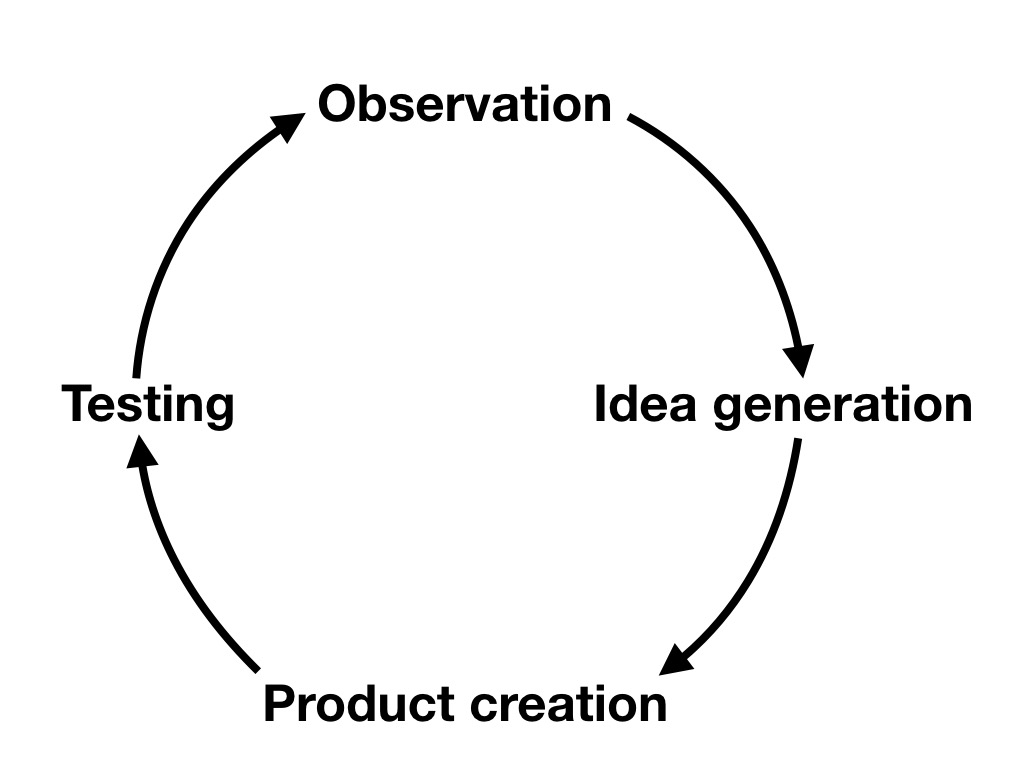
\includegraphics[width=0.5\textwidth]{ProductCreation}
\caption{Redogörelse för de fyra stegen i designprocessen vid användning av Kibana.}
\end{figure}

\begin{table}[h!]
  \begin{center}
  \caption{Sammanställning av UX-designprocessens genomförande.}
    \label{tab:table1}
 \begin{tabular}{|p{3cm}|p{3cm}|p{3cm}|p{3cm}|}
      \hline
     \textbf{Designkrav} & \textbf{Lösningar} & \textbf{Visualisering} & \textbf{Fält}\\
     \hline
  \multirow{3}{3cm}{Hur många bilar åker igenom varje betalstation och/ eller stad?} &  Trafikintensitet baserad på stad & Taggmoln  & SkatteObjekt\\\cline{2-4}
  & \multirow{2}{3cm}{Trafikintensitet baserad på betalstationer} & Karta med koordinater
& Geografisk Placering\\\cline{3-4}  
  & &  Taggmoln
& Betalstationer \\ \hline


  \multirow{2}{3cm}{Varifrån kommer bilar som åker genom betalstationerna?} &  Kommun där fordonsägare bor & Karta med geografiska områden  & Kommun\\\cline{2-4}
  &Län där fordonsägare bor
 & Karta med geografiska områden  & Län\\ \hline
 
Hur många fordon som passerade den senaste minuten? &Antal fordon
 & Antal  & PassageObjekt\\ \hline
 
 \multirow{2}{3cm}{Hur ser trafikfördelningen ut baserad på riktning?} &  Riktnings-fördelning&Cirkeldiagram& Riktning\\\cline{2-4}
  &Körfälts-fördelning 
 & Cirkeldiagram  & Körfält\\ \hline
 
 \multirow{2}{3cm}{Vilken är den mest populära fordonstypen?} &  Trafikintensitet baserad på fordonstyp & Cirkeldiagram& Fordonstyp\\\cline{2-4}
  &Trafikintensitet baserad på fordonstyp för de mest populära betalstationerna 
 & Stapeldiagram  & TidsStämpel, Betalstation, Fordonstyp\\ \hline


\end{tabular}
\end{center}
\end{table}

\chapter{Analys och diskussion}
Analys och diskussion
\blindtext


\chapter{Slutsatser}
Slutsatser
\blindtext

\chapter{Källförteckning}
Källförteckningen.


\chapter{Bilagor}

\begin{appendices}
  \chapter{First appendix}
  \section{First section}
  \section{Second section}

  \chapter{Second appendix}
  \section{First section}
  \section{Second section}
\end{appendices}
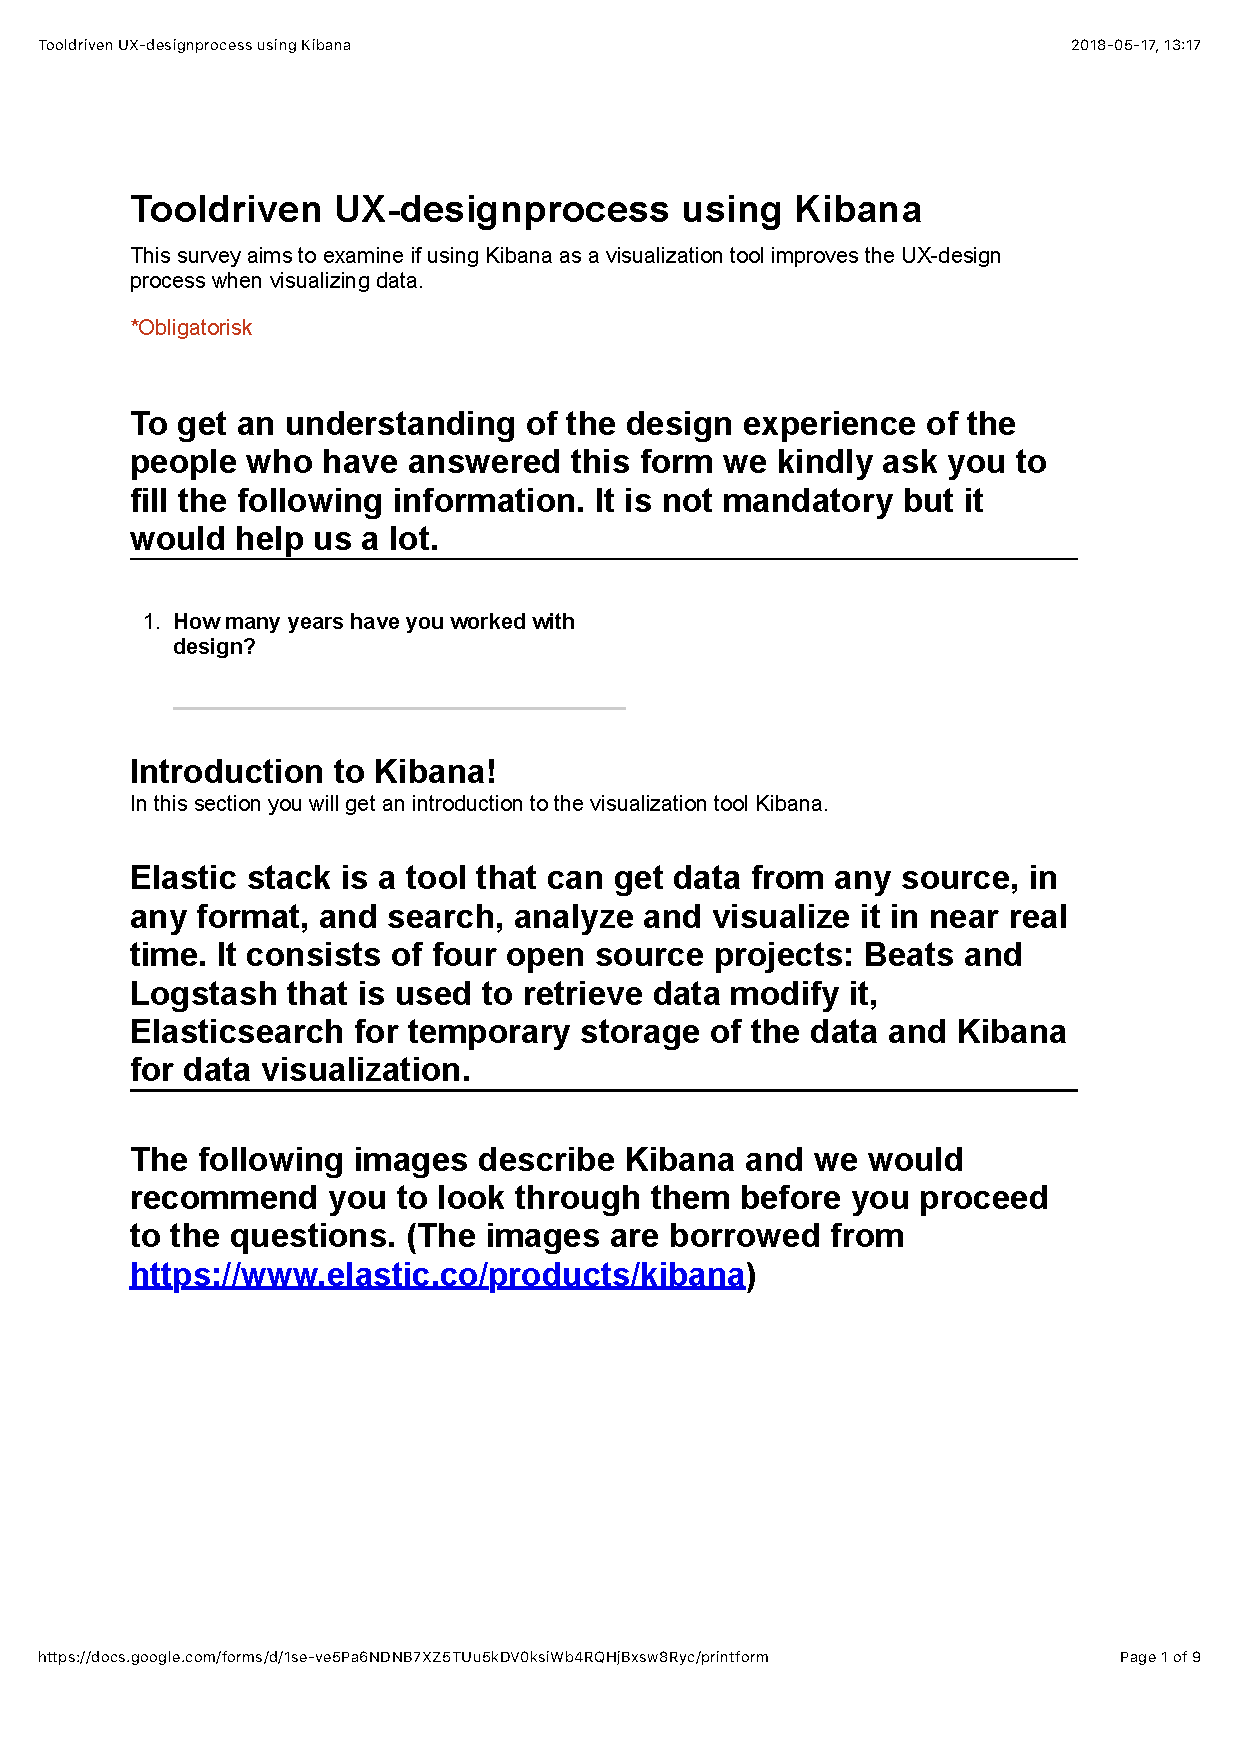
\includepdf[pages={-}]{UX_designprocess.pdf}


\end{document}
